% LaTeX body content for Part I, Chapters 4-6
% Research Companion Guide - CNN Strong Gravitational Lens Finding
% No preamble, no \part, no \begin{document} - start with \section

\section{Chapter 4: Statistics Toolkit}

This chapter explains the statistical tools we use to evaluate our CNN lens finder and to diagnose whether our simulated lens injections look realistic. We build each concept from first principles and include worked examples so you can follow the logic step by step.

\subsection{The ROC Curve and AUC}

\subsubsection{What Is a Classifier Threshold?}

When a CNN looks at an image, it outputs a \textbf{score}---a number between 0 and 1---that represents how confident it is that the image shows a strong lens. But a score alone does not make a decision. We need a \textbf{threshold}: a cutoff value $p^*$ such that we call everything with score $\geq p^*$ a ``positive'' (lens) and everything below a ``negative'' (non-lens).

For example, if $p^* = 0.5$, then any image with score $\geq 0.5$ is classified as a lens. If $p^* = 0.9$, we are stricter: only very high scores count as lenses. Changing the threshold changes how many lenses we find and how many false alarms we accept. There is a trade-off: lower thresholds find more real lenses but also more false positives; higher thresholds miss more lenses but reduce false alarms.

\subsubsection{True Positive Rate and False Positive Rate}

At each threshold $p^*$, we can compute two key rates:

\begin{itemize}
    \item \textbf{True Positive Rate (TPR)}, also called \textbf{recall}: Of all the actual lenses in our data, what fraction did we correctly classify as lenses? If we have 100 real lenses and we correctly flag 80 of them, TPR $= 80/100 = 0.80$. Higher TPR means we are finding more of the real lenses.
    \item \textbf{False Positive Rate (FPR)}: Of all the actual non-lenses, what fraction did we wrongly classify as lenses? If we have 1000 non-lenses and 50 of them got high scores and were falsely flagged, FPR $= 50/1000 = 0.05$. Lower FPR means fewer false alarms.
\end{itemize}

As we sweep $p^*$ from 0 to 1, TPR and FPR change. At $p^* = 0$, we call everything a lens, so TPR $= 1$ and FPR $= 1$. At $p^* = 1$, we call almost nothing a lens, so TPR $\approx 0$ and FPR $\approx 0$. In between, we trace out a curve.

\subsubsection{The ROC Curve}

The \textbf{ROC curve} (Receiver Operating Characteristic curve) is a plot of TPR on the vertical axis versus FPR on the horizontal axis, as we sweep the threshold from 0 to 1. Each point on the curve corresponds to one choice of threshold.

A perfect classifier would have TPR $= 1$ and FPR $= 0$ at some threshold: it finds all lenses and zero false alarms. That would trace a curve that goes straight up the left side and then across the top. A useless classifier that randomly guesses would give points along the diagonal line from $(0,0)$ to $(1,1)$: increasing the threshold trades TPR and FPR one-for-one, like flipping a coin.

\subsubsection{AUC: Area Under the Curve}

The \textbf{AUC} (Area Under the ROC Curve) is the area under the ROC curve. It is a single number that summarizes the classifier's performance across all thresholds.

\begin{itemize}
    \item \textbf{AUC $= 1.0$}: Perfect separation. The curve hugs the top-left corner; there exists a threshold where we get all lenses and no false alarms.
    \item \textbf{AUC $= 0.5$}: Random guessing. The curve lies on the diagonal; the classifier adds no information beyond chance.
    \item \textbf{AUC between 0.5 and 1.0}: Some discrimination. The higher the AUC, the better the classifier at ranking lenses above non-lenses.
\end{itemize}

\subsubsection{Intuitive Interpretation of AUC}

A beautiful interpretation: \textbf{AUC is the probability that a randomly chosen positive (lens) gets a higher score than a randomly chosen negative (non-lens)}. If we pick one lens and one non-lens at random and compare their scores, AUC tells us how often the lens wins. AUC $= 0.5$ means they tie on average (random); AUC $= 1.0$ means the lens always wins; AUC $= 0.8$ means the lens wins 80\% of the time.

\begin{figure}[htbp]
\centering
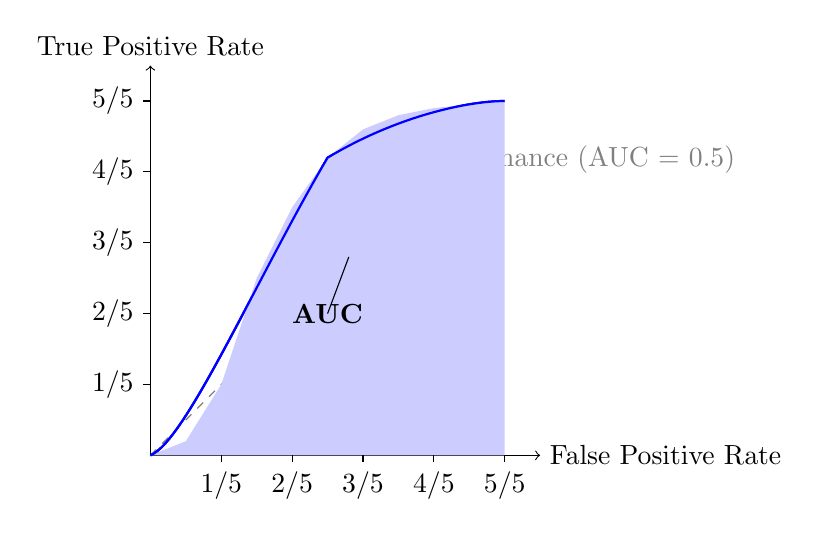
\begin{tikzpicture}[scale=0.9]
    % Axes
    \draw[->] (0,0) -- (5.5,0) node[right] {False Positive Rate};
    \draw[->] (0,0) -- (0,5.5) node[above] {True Positive Rate};
    
    % Chance diagonal
    \draw[dashed, gray] (0,0) -- (5,5) node[pos=0.9, below right] {Chance (AUC = 0.5)};
    
    % ROC curve (concave, typical good classifier)
    \draw[thick, blue] (0,0) .. controls (0.5,0.2) and (1.5,2.5) .. (2.5,4.2) .. controls (3.5,4.8) and (4.5,5) .. (5,5);
    
    % Shaded area under ROC curve (AUC)
    \fill[blue!20] (0,0) -- (0.5,0.2) -- (1,1) -- (1.5,2.5) -- (2,3.5) -- (2.5,4.2) -- (3,4.6) -- (3.5,4.8) -- (4,4.9) -- (4.5,4.95) -- (5,5) -- (5,0) -- cycle;
    
    % Redraw curve on top of fill
    \draw[thick, blue] (0,0) .. controls (0.5,0.2) and (1.5,2.5) .. (2.5,4.2) .. controls (3.5,4.8) and (4.5,5) .. (5,5);
    
    % Labels
    \node at (2.5,2) {\textbf{AUC}};
    \draw (2.5,2) -- (2.8,2.8);
    
    % Tick marks
    \foreach \x in {1,2,3,4,5} {
        \draw (\x,0) -- (\x,-0.1) node[below] {\x/5};
        \draw (0,\x) -- (-0.1,\x) node[left] {\x/5};
    }
\end{tikzpicture}
\caption{An ROC curve. The blue curve shows TPR vs FPR as the classifier threshold is swept. The shaded area under the curve is the AUC. The dashed diagonal represents chance performance (AUC = 0.5).}
\end{figure}

\subsection{Logistic Regression as a ``Linear Probe''}

\subsubsection{What Is Logistic Regression?}

\textbf{Logistic regression} is a simple statistical model that finds a \textbf{flat hyperplane} in a high-dimensional space to separate two groups. In 2D, a hyperplane is a straight line; in 3D, it is a flat plane; in many dimensions, it is still ``flat''---no curves, no bends. The model learns weights such that one side of the hyperplane tends to have positives and the other side negatives.

\subsubsection{Why ``Linear''?}

``Linear'' means the decision boundary is a straight line (in 2D) or a flat hyperplane (in higher dimensions). The model cannot draw curved boundaries. If the two groups are arranged in a circle versus everything inside, a linear classifier would struggle. If they are separated by a straight cut, a linear classifier excels.

\subsubsection{Using It as a Probe}

In our paper, we do \emph{not} use logistic regression to build a new lens finder. We use it as a \textbf{diagnostic probe}: we take the internal representations (embeddings) that the CNN produces for each image and ask, ``Can a simple linear classifier separate real lenses from parametric injections using just these embeddings?''

If the answer is yes---if logistic regression achieves AUC near 1.0---then the two groups are \textbf{trivially separable} in that feature space. The CNN's internal representation makes it easy to tell them apart with a straight cut. That means the parametric injections do \emph{not} look like real lenses to the CNN; they occupy a different region of feature space.

If the answer is no---if logistic regression gets AUC near 0.5---then the two groups overlap. The CNN cannot easily tell them apart with a linear boundary, which suggests the injections may be more realistic.

It is called a ``probe'' because we are \emph{probing} what the CNN has learned, not training a new classifier from scratch. The CNN is already trained; we are just inspecting its feature space.

\subsection{Cross-Validation (k-Fold)}

\subsubsection{Why Not Test on Training Data?}

If we train a model on a dataset and then evaluate it on the \emph{same} data, we get an overly optimistic result. The model has already ``seen'' those examples and can memorize them. This is called \textbf{overfitting}. To get an honest estimate of performance, we must test on data the model has never seen.

\subsubsection{The k-Fold Procedure}

\textbf{k-fold cross-validation} splits the data into $k$ equal parts (folds). We do $k$ rounds:

\begin{enumerate}
    \item Round 1: Train on folds 2, 3, 4, 5; test on fold 1.
    \item Round 2: Train on folds 1, 3, 4, 5; test on fold 2.
    \item Round 3: Train on folds 1, 2, 4, 5; test on fold 3.
    \item Round 4: Train on folds 1, 2, 3, 5; test on fold 4.
    \item Round 5: Train on folds 1, 2, 3, 4; test on fold 5.
\end{enumerate}

Each fold serves as the test set exactly once. We rotate through all folds so every data point is used for testing once. We report the \textbf{mean} and \textbf{standard deviation} of the metric (e.g., AUC) across the $k$ folds. The mean gives our best estimate; the standard deviation tells us how stable the result is.

\subsubsection{In Our Paper}

We use 5-fold cross-validation with 112 real lens embeddings and 500 parametric injection embeddings. Each fold has roughly 90\% for training and 10\% for testing. We report mean AUC and its standard deviation across the 5 folds. This ensures our linear probe result is not due to a lucky split of the data.

\begin{figure}[htbp]
\centering
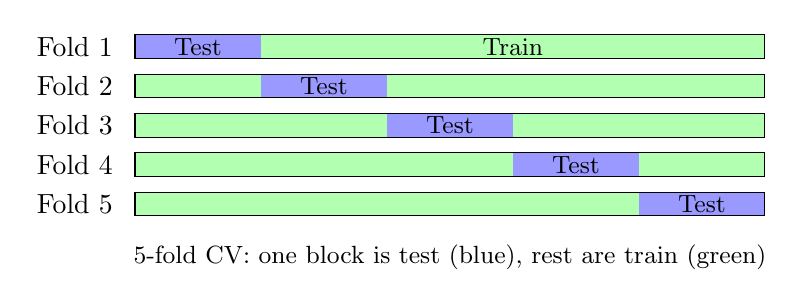
\begin{tikzpicture}[x=0.8cm, y=0.5cm]
    % Fold 1: block 1 test, blocks 2-5 train
    \fill[blue!40] (0,5) rectangle (2,5.6);
    \fill[green!30] (2,5) rectangle (10,5.6);
    \draw (0,5) rectangle (10,5.6);
    \node[left] at (-0.2, 5.3) {Fold 1};
    \node at (1, 5.3) {\small Test};
    \node at (6, 5.3) {\small Train};
    % Fold 2: block 2 test
    \fill[green!30] (0,4) rectangle (2,4.6);
    \fill[blue!40] (2,4) rectangle (4,4.6);
    \fill[green!30] (4,4) rectangle (10,4.6);
    \draw (0,4) rectangle (10,4.6);
    \node[left] at (-0.2, 4.3) {Fold 2};
    \node at (3, 4.3) {\small Test};
    % Fold 3: block 3 test
    \fill[green!30] (0,3) rectangle (4,3.6);
    \fill[blue!40] (4,3) rectangle (6,3.6);
    \fill[green!30] (6,3) rectangle (10,3.6);
    \draw (0,3) rectangle (10,3.6);
    \node[left] at (-0.2, 3.3) {Fold 3};
    \node at (5, 3.3) {\small Test};
    % Fold 4: block 4 test
    \fill[green!30] (0,2) rectangle (6,2.6);
    \fill[blue!40] (6,2) rectangle (8,2.6);
    \fill[green!30] (8,2) rectangle (10,2.6);
    \draw (0,2) rectangle (10,2.6);
    \node[left] at (-0.2, 2.3) {Fold 4};
    \node at (7, 2.3) {\small Test};
    % Fold 5: block 5 test
    \fill[green!30] (0,1) rectangle (8,1.6);
    \fill[blue!40] (8,1) rectangle (10,1.6);
    \draw (0,1) rectangle (10,1.6);
    \node[left] at (-0.2, 1.3) {Fold 5};
    \node at (9, 1.3) {\small Test};
    \node[below, font=\small] at (5, 0.5) {5-fold CV: one block is test (blue), rest are train (green)};
\end{tikzpicture}
\caption{Schematic of 5-fold cross-validation. Each horizontal bar represents one round. The blue block is the test set; the green blocks are the training set. The test block rotates across the five rounds.}
\end{figure}

\subsection{Confidence Intervals}

A point estimate (e.g., ``recall is 80\%'') is useful, but we also want to know how precise it is. \textbf{Confidence intervals} give a range of plausible values. We use two types.

\subsubsection{Wilson Score Interval for Proportions}

When we estimate a proportion (e.g., recall $= \frac{\text{recovered}}{\text{injected}}$), the naive formula $\hat{p} \pm z \sqrt{\hat{p}(1-\hat{p})/n}$ works poorly for small samples or proportions near 0 or 1. The \textbf{Wilson score interval} is a formula that accounts for this and produces more reliable intervals. It is what we use for recall and other proportions in the paper.

\subsubsection{Bootstrap Confidence Intervals for AUC}

For AUC, we use the \textbf{bootstrap}:

\begin{enumerate}
    \item Resample the data \emph{with replacement} to get a new dataset of the same size (some points appear multiple times, some not at all).
    \item Compute AUC on this resampled dataset.
    \item Repeat many times (e.g., 1000 or 10,000).
    \item The bootstrap distribution of AUC approximates the sampling distribution. A 95\% confidence interval is the 2.5th to 97.5th percentile of this distribution.
\end{enumerate}

The bootstrap makes minimal assumptions about the underlying distribution and is widely used for complex statistics like AUC.

\subsection{Permutation Tests}

\subsubsection{The Logic}

\textbf{Permutation testing} answers: ``If there were really no difference between the two groups, how often would we see a result as extreme as ours by chance?'' The key idea: \emph{if the groups are the same, then shuffling the labels should not change the result}. We can simulate this by randomly reassigning ``lens'' and ``non-lens'' labels and recomputing our statistic (e.g., AUC) each time.

\subsubsection{The Procedure}

\begin{enumerate}
    \item Compute the observed test statistic (e.g., AUC $= 0.997$ for separating real lenses from parametric injections).
    \item Shuffle the labels: randomly swap ``lens'' and ``injection'' among the 612 embeddings. The scores stay attached to each embedding; only the labels change.
    \item Train the linear probe on the shuffled data and compute AUC.
    \item Repeat step 2--3 many times (e.g., 1000 permutations).
    \item The \textbf{p-value} is the fraction of permutations where the permuted AUC $\geq$ observed AUC (plus a small correction, e.g., add 1 to numerator and denominator, to avoid p-value $= 0$).
\end{enumerate}

If the observed AUC (0.997) is far to the right of the permutation distribution (centered near 0.5), then very few---or zero---permutations beat it. The p-value is tiny. We conclude that the separation is statistically significant: it is extremely unlikely to arise by chance if the two groups were the same.

\subsubsection{Why Permutation Tests Are Powerful}

Permutation tests make \textbf{no assumptions} about the distribution of the data. They do not require normality or any parametric model. They are exact (or nearly exact) for the null hypothesis that the labels are exchangeable. They are ideal when we have a complex statistic like AUC and want a nonparametric test.

\begin{figure}[htbp]
\centering
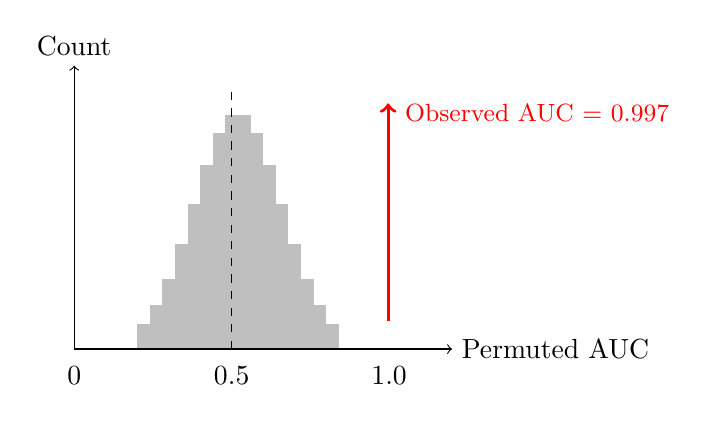
\begin{tikzpicture}[x=4cm, y=1.2cm]
    % Histogram bars (permutation distribution centered at 0.5)
    \foreach \i in {0,...,15} {
        \pgfmathsetmacro{\x}{0.2 + \i*0.04}
        \pgfmathsetmacro{\h}{2.5*exp(-25*(\x-0.5)*(\x-0.5))}
        \fill[gray!50] (\x, 0) rectangle (\x+0.04, \h);
    }
    % Axes
    \draw[->] (0,0) -- (1.2,0) node[right] {Permuted AUC};
    \draw[->] (0,0) -- (0,3) node[above] {Count};
    % Red arrow at observed AUC (0.997 off scale, in margin)
    \draw[red, very thick, ->] (0.997, 0.3) -- (0.997, 2.6);
    \node[red, right, font=\small] at (1.02, 2.5) {Observed AUC = 0.997};
    % Vertical dashed line at 0.5
    \draw[dashed] (0.5, 0) -- (0.5, 2.8);
    \node[below] at (0.5, -0.08) {0.5};
    \node[below] at (0, -0.08) {0};
    \node[below] at (1.0, -0.08) {1.0};
\end{tikzpicture}
\caption{Permutation test. The gray histogram shows the distribution of AUC when labels are randomly shuffled (centered near 0.5). The red arrow marks our observed AUC (0.997). Almost no permutations reach that value, so the p-value is extremely small.}
\end{figure}

\subsection{Fr\'echet Distance}

The \textbf{Fr\'echet distance} (sometimes called the Fr\'echet Inception Distance in machine learning) measures how different two probability distributions are in high-dimensional space. Given two sets of points (e.g., embeddings from real lenses vs parametric injections), we compute the mean and covariance matrix of each set. The Fr\'echet distance combines the difference between the means and the difference between the covariances into a single number.

\textbf{Larger Fr\'echet distance} = the two distributions are more different. Smaller = more similar. It is useful for comparing whether two sets of embeddings occupy similar regions of feature space.

\textbf{Caveat}: When the sample size is smaller than the dimensionality (e.g., 112 embeddings in a 512-dimensional space), the covariance matrix becomes \textbf{singular} (not invertible). The Fr\'echet distance formula breaks down. It is unreliable in such cases, so we must be careful when interpreting it for small datasets.

\subsection{Understanding p-Values}

A \textbf{p-value} answers: ``If the null hypothesis were true (e.g., there is no difference between groups), what is the probability of observing a result as extreme as ours---or more extreme---just by chance?''

\textbf{What p-values mean}: A small p-value (e.g., $p < 0.05$) means that such an extreme result would be rare if the null were true. So we have evidence against the null; we may reject it.

\textbf{What p-values do NOT mean}: A p-value is \emph{not} the probability that the null hypothesis is true. It is \emph{not} the probability that our result is a fluke. It assumes the null is true and asks how often we would see data this weird. This is a subtle but crucial distinction.

\subsection{Comparing Two Proportions: The Two-Proportion z-Test}

When we compare two percentages (e.g., completeness of 5.18\% vs 3.79\%), we use a \textbf{two-proportion z-test}. We compute a z-statistic based on the difference between the two proportions and their combined standard error. Under the null hypothesis that the two proportions are equal, this z-statistic follows (approximately) a standard normal distribution. We can then compute a p-value.

For example, if we find 5.18\% completeness in one sample and 3.79\% in another, the z-test tells us whether that difference is statistically significant or could easily have arisen by chance.

\subsection{The Sign Test}

When we have \textbf{paired} binary outcomes (e.g., for each of 112 lenses, we have two classifications: ``found by method A'' and ``found by method B''), the \textbf{sign test} compares the two methods. For each pair, we note whether A and B agree or disagree. We count how many times A found a lens when B did not, and vice versa. Under the null that the two methods are equally good, we expect roughly equal numbers in each direction. The sign test uses the binomial distribution to compute how unlikely an imbalance is. It is simple, nonparametric, and does not assume normality.

\bigskip
\noindent\textit{We use these tools throughout the paper: AUC and the linear probe to diagnose injection realism, cross-validation for robust estimates, permutation tests for significance, and confidence intervals and proportion tests to compare completeness and recall across methods.}

\newpage
\section{Chapter 5: The DESI Legacy Imaging Survey}

The images we use for finding strong lenses come from the \textbf{DESI Legacy Imaging Survey}. This section explains what that survey is, what its data look like, and why these choices matter for our analysis.

\subsection{What Is DESI?}

\textbf{DESI} stands for the \textbf{Dark Energy Spectroscopic Instrument}. It is a large spectroscopic survey designed to measure the distances and velocities of tens of millions of galaxies and quasars. Its goal is to map the large-scale structure of the universe and constrain dark energy---the mysterious component causing cosmic acceleration.

DESI needs a catalog of targets to observe: galaxies and quasars with positions, brightnesses, and colors. That catalog comes from \textbf{imaging}---taking pictures of the sky in several bands. DESI does not do its own imaging; it uses data from the \textbf{Legacy Imaging Surveys}, which were specifically designed to support DESI target selection.

\subsection{Data Release 10 (DR10)}

\textbf{DR10} is the \textbf{Data Release 10}---the tenth public release of the Legacy Imaging Survey data. Each release incorporates new observations, improved processing, and refined calibrations. DR10 represents the state of the data at the time of our analysis. It combines imaging from three surveys: the \textbf{Dark Energy Camera Legacy Survey} (DECaLS), the \textbf{Beijing-Arizona Sky Survey} (BASS), and the \textbf{Mayall z-band Legacy Survey} (MzLS). Together they cover the extragalactic sky visible from the northern hemisphere.

\subsection{The Three Optical Bands}

The Legacy Survey observes in three optical bands:

\begin{itemize}
    \item \textbf{g band} (blue-green): Central wavelength $\sim 475$ nm. Sensitive to younger, bluer stellar populations and star-forming regions.
    \item \textbf{r band} (red): Central wavelength $\sim 622$ nm. Often the ``fiducial'' band for morphology; good balance of depth and resolution.
    \item \textbf{z band} (near-infrared): Central wavelength $\sim 913$ nm. Probes redder, older stellar light; less affected by dust extinction.
\end{itemize}

Together, g, r, and z provide \textbf{color} information. The ratio of flux in different bands tells us about stellar populations, dust, and redshift. For strong lenses, the lens galaxy is typically an old, red elliptical, while the background source can be bluer. Color helps distinguish lenses from non-lenses.

\subsection{Pixel Scale: What Does 0.262 Arcsec Mean?}

The \textbf{pixel scale} is 0.262 arcsec per pixel. An \textbf{arcsecond} is $1/3600$ of a degree---a very small angle. The full Moon is about 1800 arcsec across, so one arcsecond is roughly 1/1800 of the Moon's diameter.

At typical lens redshifts ($z \sim 0.3$--0.5), 1 arcsec corresponds to about 3--5 \textbf{kiloparsecs} (kpc). A kiloparsec is about 3260 light-years, so 1 arcsec spans roughly 10,000--16,000 light-years at these distances. That means each pixel (0.262 arcsec) corresponds to about 800--4000 light-years. The pixel scale sets the smallest spatial features we can resolve.

\subsection{Depth: How Faint Can We See?}

\textbf{Depth} describes how faint an object can be and still be detected. Surveys quote \textbf{5-sigma depth}: the magnitude at which a point source is detected with 5-sigma significance (i.e., the signal is 5 times the noise). For the Legacy Survey, typical 5-sigma depths are:

\begin{itemize}
    \item g $\sim 24.7$ mag
    \item r $\sim 23.9$ mag
    \item z $\sim 23.0$ mag
\end{itemize}

Each magnitude step of 1 corresponds to a factor of about 2.5 in brightness (on the logarithmic magnitude scale). So mag 24 is about 2.5 times fainter than mag 23, and about $2.5^4 \approx 40$ times fainter than mag 20. The brightest stars visible to the naked eye are around mag 6. Mag 24 is roughly $2.5^{18} \approx 100$ million times fainter. These depths allow us to detect distant lensed galaxies that would be invisible in shallower surveys.

\subsection{Seeing: Atmospheric Blurring}

\textbf{Seeing} refers to the blurring of images by Earth's atmosphere. Turbulent air cells deflect light, so a point source spreads into a blob. The \textbf{point spread function} (PSF) describes this blur. Its width is often quantified by the \textbf{FWHM} (Full Width at Half Maximum): the diameter of the blob at half its peak brightness.

The median seeing in the r-band is about 1.3 arcsec. That means features smaller than $\sim 1.3$ arcsec are blurred together. Strong lens arcs can be a few arcseconds long, so they are marginally resolved. Better seeing (smaller FWHM) would sharpen the arcs; worse seeing would smear them further.

\subsection{Nanomaggies: The Flux Unit}

The Legacy Survey reports flux in \textbf{nanomaggies}. One nanomaggy corresponds to AB magnitude 22.5. The conversion is:
\begin{equation}
\text{flux}_{\text{nanomaggy}} = 10^{(22.5 - \text{magnitude})/2.5}
\end{equation}
So magnitude 22.5 gives 1 nanomaggy; magnitude 20 gives $10^{1} = 10$ nanomaggies; magnitude 25 gives $10^{-1} = 0.1$ nanomaggies. Working in linear flux (nanomaggies) is convenient for modeling and for combining bands.

\subsection{Cutouts: Our 101$\times$101 Pixel Images}

We do not use full survey images. We extract \textbf{cutouts}: small square regions centered on each galaxy of interest. Our cutouts are 101$\times$101 pixels.

With 0.262 arcsec per pixel, 101 pixels span $101 \times 0.262 \approx 26.5$ arcsec on a side. So each cutout covers about $26.5 \times 26.5$ square arcseconds. This is large enough to capture the lens galaxy, any lensed arcs, and surrounding sky; it is small enough to be computationally manageable and to avoid too much contamination from neighboring objects.

\subsection{Survey Coverage}

The Legacy Imaging Survey covers approximately 14,000 square degrees of sky---about one-third of the entire sky. This is the northern extragalactic sky, avoiding the plane of the Milky Way where dust and stars would contaminate the data. The large area means we have many galaxies to search for lenses, but it also means we rely on automated methods like CNNs to process the data.

\bigskip
\noindent\textit{In summary: We use DR10 cutouts in g, r, and z bands, with 0.262 arcsec pixels, depth to mag $\sim$24, and seeing $\sim$1.3 arcsec. These choices match the real survey conditions under which our CNN was trained and will be applied.}

\newpage
\section{Chapter 6: Prior Work This Paper Builds On}

Our paper did not arise in a vacuum. Several earlier studies laid the groundwork and identified key limitations. This chapter summarizes each contribution and the gap that our work fills.

\subsection{Herle et al.\ (2024): Biases in CNN Detection}

\textbf{Reference:} Herle et al., MNRAS \textbf{534}, 1093 (2024).

Herle and collaborators studied how a CNN lens finder's \textbf{detection probability} depends on lens and source properties. They varied the Einstein radius (a measure of lens strength), the S\'ersic index (a measure of how ``concentrated'' the lens galaxy light is), and the source size. Using \textbf{simulated Euclid-like data}---space-based imaging with higher resolution than ground-based surveys---they trained a CNN and measured its detection rate as a function of these parameters.

\textbf{Key finding:} Detection is \textbf{strongly biased}. The CNN preferentially finds certain types of lenses: those with larger Einstein radii, particular S\'ersic indices, and certain source sizes. Lenses that fall outside these ``sweet spots'' are missed more often. In other words, the CNN has a \textbf{selection function} that is not uniform across lens parameter space.

\textbf{Limitation:} Herle et al.\ worked entirely in simulation. They never compared their simulated lenses to real confirmed lenses. So they demonstrated that the selection function is biased in a simulated world, but they could not say whether those simulated lenses look \emph{realistic} to the CNN. If the simulations are wrong, the inferred bias may not apply to the real universe. Our paper directly addresses that gap by comparing real lenses to simulated injections in the CNN's feature space.

\subsection{Canameras et al.\ (2024, HOLISMOKES XI): Real-Galaxy Sources}

\textbf{Reference:} Canameras et al., A\&A \textbf{692}, A72 (2024)---HOLISMOKES XI.

Canameras and collaborators took a different approach to realism. Instead of using \textbf{parametric models} (e.g., S\'ersic profiles) for the background source galaxies, they used \textbf{real galaxy images} from the \textbf{Hubble Ultra Deep Field} (HUDF). They ``injected'' these real-galaxy sources into \textbf{Hyper Suprime-Cam} (HSC) survey imaging---a different telescope and survey from the Legacy Survey, but also ground-based optical imaging.

\textbf{Key contribution:} They explicitly noted that \textbf{S\'ersic profiles are inadequate} for modeling real sources. Real galaxies have irregular shapes, spiral arms, clumps, and asymmetric structure. A smooth S\'ersic ellipse cannot capture that. By using real HUDF galaxies, they bypassed the parametric limitation entirely.

\textbf{Limitation:} They did \emph{not} quantify how different parametric and real injections look in the CNN's internal representation. Their observation was qualitative: real galaxies look more realistic. Our paper provides a \textbf{quantitative} diagnostic: we measure the linear probe AUC between real lenses and parametric injections in embedding space. We show that the difference is large (AUC $\approx$ 0.997) and statistically significant. We also propose this as a tool the community can use to evaluate any injection scheme.

\subsection{Collett \& Cunnington (2022): The Injection-Recovery Framework}

\textbf{Reference:} Collett \& Cunnington, MNRAS \textbf{516}, 1808 (2022).

Collett and Cunnington established the \textbf{injection-recovery framework} for calibrating CNN lens finder selection functions. The idea: simulate lenses by injecting synthetic lensed sources into real survey images, run the CNN on the result, and measure the recovery fraction. This gives an empirically calibrated completeness curve: at each lens parameter value, what fraction of injected lenses does the CNN find?

They used \textbf{parametric models}: a singular isothermal ellipse (SIE) for the lens and a S\'ersic profile for the source. Their methodology is foundational---it is the standard approach in the field. Our paper builds on this framework but asks: do parametric injections produce the same recovery statistics as real lenses would? If not, the calibration may be wrong. Our linear probe provides a way to test that.

\subsection{Huang et al.\ (2020): The DECaLS Lens Catalog}

\textbf{Reference:} Huang et al., ApJ \textbf{894}, 78 (2020).

Huang and collaborators applied a \textbf{ResNet} CNN to find strong lens candidates in the DECaLS survey---a predecessor to and component of the Legacy Survey DR10. They produced a large catalog of candidates and released it to the community.

\textbf{Limitation:} They did \emph{not} perform injection-recovery or completeness analysis. They focused on finding candidates, not on calibrating the selection function. Our work assumes such a catalog exists (or could exist) and asks: when we calibrate it with injections, are those injections realistic enough?

\subsection{The Gap Our Paper Fills}

No prior work had done all of the following:

\begin{enumerate}
    \item \textbf{Directly measured} how different real lenses look from parametric injections in CNN feature space. Herle et al.\ used simulation only; Canameras et al.\ used real galaxies but did not quantify the difference in embedding space.
    \item \textbf{Performed a controlled experiment} to diagnose the cause. We compare real lenses to parametric injections, and real lenses to real-galaxy injections, in the same embedding space. We show that the problem is the source model (parametric vs.\ real), not the lens or the pipeline.
    \item \textbf{Proposed a quantitative diagnostic tool}---the linear probe AUC---that the community can use to evaluate any injection scheme. Before our paper, there was no standard way to ask: ``Do my injections look like real lenses to this CNN?'' Now there is.
\end{enumerate}

Our paper thus bridges the gap between simulation-based calibration (Collett \& Cunnington, Herle et al.) and the qualitative recognition that real galaxies matter (Canameras et al.). We provide a concrete, implementable test: if the linear probe AUC between real lenses and your injections is near 1.0, your injections are not realistic. If it is near 0.5, they may be. This is a step toward more reliable completeness calibration for CNN lens finders.
